\documentclass[12pt, a4paper, oneside]{article}\usepackage[]{graphicx}\usepackage[]{color}
%% maxwidth is the original width if it is less than linewidth
%% otherwise use linewidth (to make sure the graphics do not exceed the margin)
\makeatletter
\def\maxwidth{ %
  \ifdim\Gin@nat@width>\linewidth
    \linewidth
  \else
    \Gin@nat@width
  \fi
}
\makeatother

\definecolor{fgcolor}{rgb}{0.345, 0.345, 0.345}
\newcommand{\hlnum}[1]{\textcolor[rgb]{0.686,0.059,0.569}{#1}}%
\newcommand{\hlstr}[1]{\textcolor[rgb]{0.192,0.494,0.8}{#1}}%
\newcommand{\hlcom}[1]{\textcolor[rgb]{0.678,0.584,0.686}{\textit{#1}}}%
\newcommand{\hlopt}[1]{\textcolor[rgb]{0,0,0}{#1}}%
\newcommand{\hlstd}[1]{\textcolor[rgb]{0.345,0.345,0.345}{#1}}%
\newcommand{\hlkwa}[1]{\textcolor[rgb]{0.161,0.373,0.58}{\textbf{#1}}}%
\newcommand{\hlkwb}[1]{\textcolor[rgb]{0.69,0.353,0.396}{#1}}%
\newcommand{\hlkwc}[1]{\textcolor[rgb]{0.333,0.667,0.333}{#1}}%
\newcommand{\hlkwd}[1]{\textcolor[rgb]{0.737,0.353,0.396}{\textbf{#1}}}%

\usepackage{framed}
\makeatletter
\newenvironment{kframe}{%
 \def\at@end@of@kframe{}%
 \ifinner\ifhmode%
  \def\at@end@of@kframe{\end{minipage}}%
  \begin{minipage}{\columnwidth}%
 \fi\fi%
 \def\FrameCommand##1{\hskip\@totalleftmargin \hskip-\fboxsep
 \colorbox{shadecolor}{##1}\hskip-\fboxsep
     % There is no \\@totalrightmargin, so:
     \hskip-\linewidth \hskip-\@totalleftmargin \hskip\columnwidth}%
 \MakeFramed {\advance\hsize-\width
   \@totalleftmargin\z@ \linewidth\hsize
   \@setminipage}}%
 {\par\unskip\endMakeFramed%
 \at@end@of@kframe}
\makeatother

\definecolor{shadecolor}{rgb}{.97, .97, .97}
\definecolor{messagecolor}{rgb}{0, 0, 0}
\definecolor{warningcolor}{rgb}{1, 0, 1}
\definecolor{errorcolor}{rgb}{1, 0, 0}
\newenvironment{knitrout}{}{} % an empty environment to be redefined in TeX

\usepackage{alltt} % Paper size, default font size and one-sided paper
%\graphicspath{{./Figures/}} % Specifies the directory where pictures are stored
%\usepackage[dcucite]{harvard}
\usepackage{rotating}
\usepackage{amsmath}
\usepackage{setspace}
\usepackage{pdflscape}
\usepackage[flushleft]{threeparttable}
\usepackage{multirow}
\usepackage[comma, sort&compress]{natbib}% Use the natbib reference package - read up on this to edit the reference style; if you want text (e.g. Smith et al., 2012) for the in-text references (instead of numbers), remove 'numbers' 
\usepackage{graphicx}
%\bibliographystyle{plainnat}
\bibliographystyle{agsm}
\usepackage[colorlinks = true, citecolor = blue, linkcolor = blue]{hyperref}
%\hypersetup{urlcolor=blue, colorlinks=true} % Colors hyperlinks in blue - change to black if annoying
%\renewcommand[\harvardurl]{URL: \url}
\IfFileExists{upquote.sty}{\usepackage{upquote}}{}
\begin{document}
\title{Trends}
\author{Rob Hayward\footnote{University of Brighton Business School, Lewes Road, Brighton, BN2 4AT; Telephone 01273 642586.  rh49@brighton.ac.uk}}
\date{\today}
\maketitle
\section*{Introduction}
One aspects of paris tht may be investigted would be the relatonship between the two series. In the \emph{Pairs} slides in the \emph{Pair} folder, two ways of looking at the relationship were considered: the difference between share price and the ratio of share prices.  The evolution of these may be considered. 

The following is taken from \href{Arthur Charpentier}{http://freakonometrics.hypotheses.org/13287}.  

\begin{knitrout}
\definecolor{shadecolor}{rgb}{0.969, 0.969, 0.969}\color{fgcolor}\begin{kframe}
\begin{alltt}
autoroute = \hlkwd{read.table}(\hlstr{"http://freakonometrics.blog.free.fr/public/data/autoroute.csv"}, 
    header = TRUE, sep = \hlstr{";"})
X = autoroute$a100
T = 1:\hlkwd{length}(X)
\hlkwd{plot}(T, X, type = \hlstr{"l"}, xlim = \hlkwd{c}(0, 120), main = \hlstr{"French Road Trffic"})
reg = \hlkwd{lm}(X ~ T)
\hlkwd{abline}(reg, col = \hlstr{"red"})
\end{alltt}
\end{kframe}
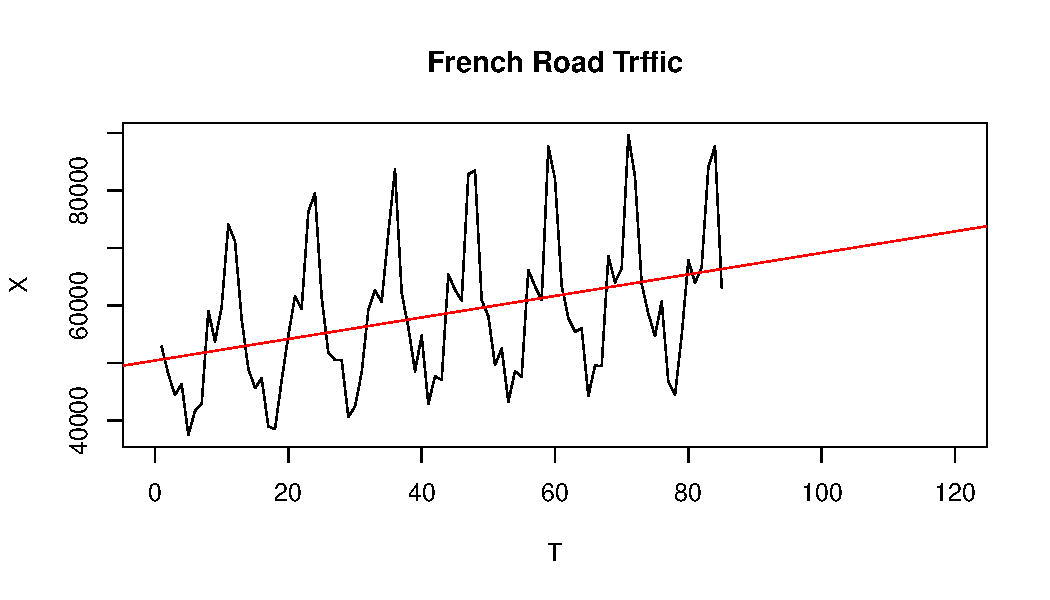
\includegraphics[width=\maxwidth]{figure/Plot} 

\end{knitrout}

It is possible to work on the residuals from the regression. $Y = X_t - (a + bt)$.
\begin{knitrout}
\definecolor{shadecolor}{rgb}{0.969, 0.969, 0.969}\color{fgcolor}\begin{kframe}
\begin{alltt}
Y = \hlkwd{residuals}(reg)
\hlkwd{acf}(Y, lag = 36, lwd = 3)
\end{alltt}
\end{kframe}
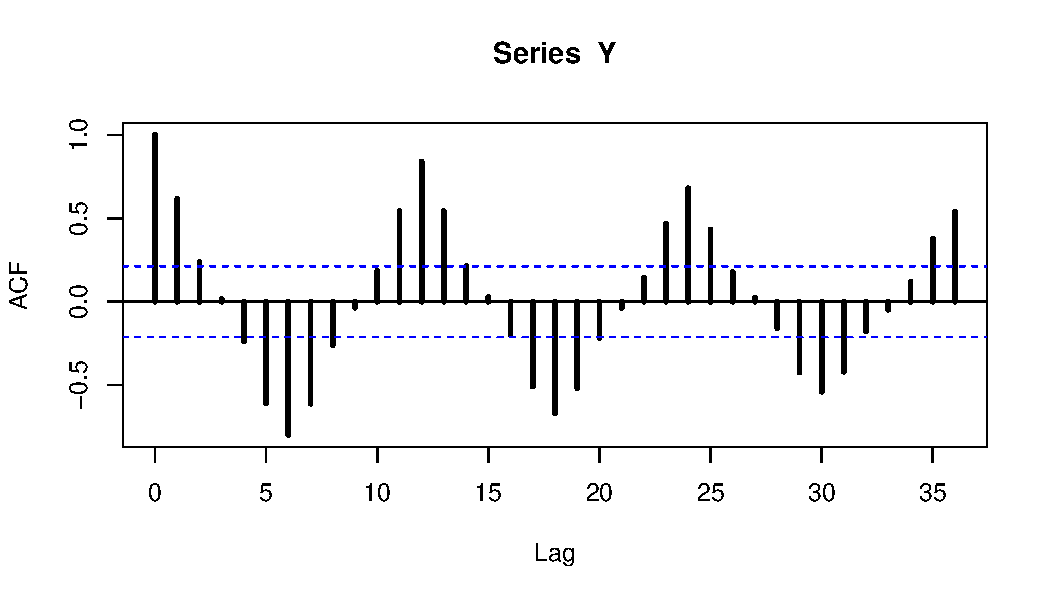
\includegraphics[width=\maxwidth]{figure/Resid} 

\end{knitrout}

There appers to be a seasonal pattern. Therefore, create $Z_t = (1 - L^{12})Y_t$.  The ACF.
\begin{knitrout}
\definecolor{shadecolor}{rgb}{0.969, 0.969, 0.969}\color{fgcolor}\begin{kframe}
\begin{alltt}
Z = \hlkwd{diff}(Y, 12)
\hlkwd{acf}(Z, lag = 36, lwd = 3)
\end{alltt}
\end{kframe}
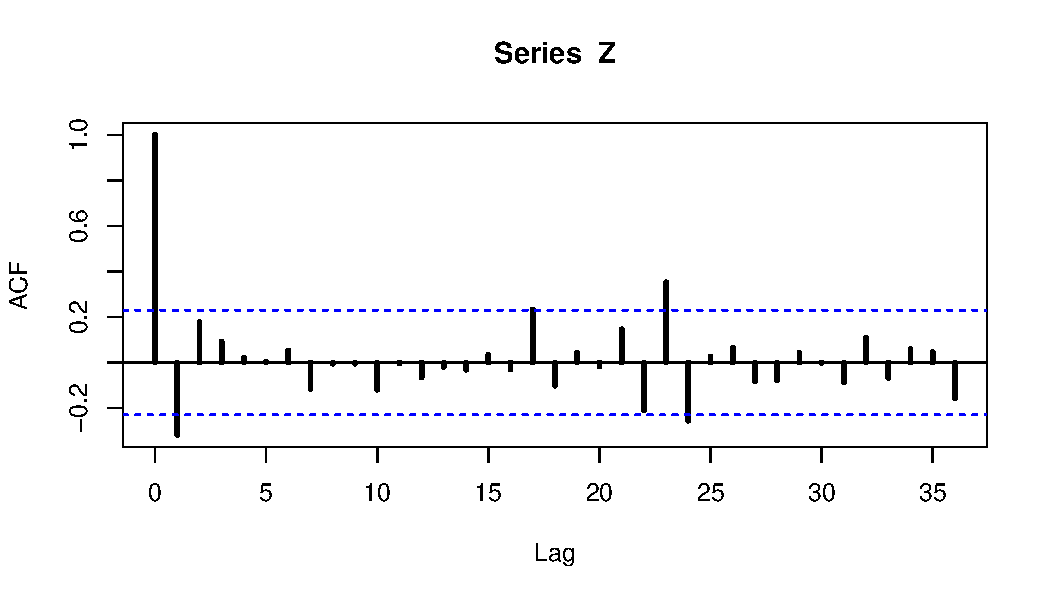
\includegraphics[width=\maxwidth]{figure/cf} 

\end{knitrout}

Arthur suggests that this suggests a MA(1) pattern. 

The PCF
\begin{knitrout}
\definecolor{shadecolor}{rgb}{0.969, 0.969, 0.969}\color{fgcolor}\begin{kframe}
\begin{alltt}
\hlkwd{pacf}(Z, lag = 36, lwd = 3)
\end{alltt}
\end{kframe}
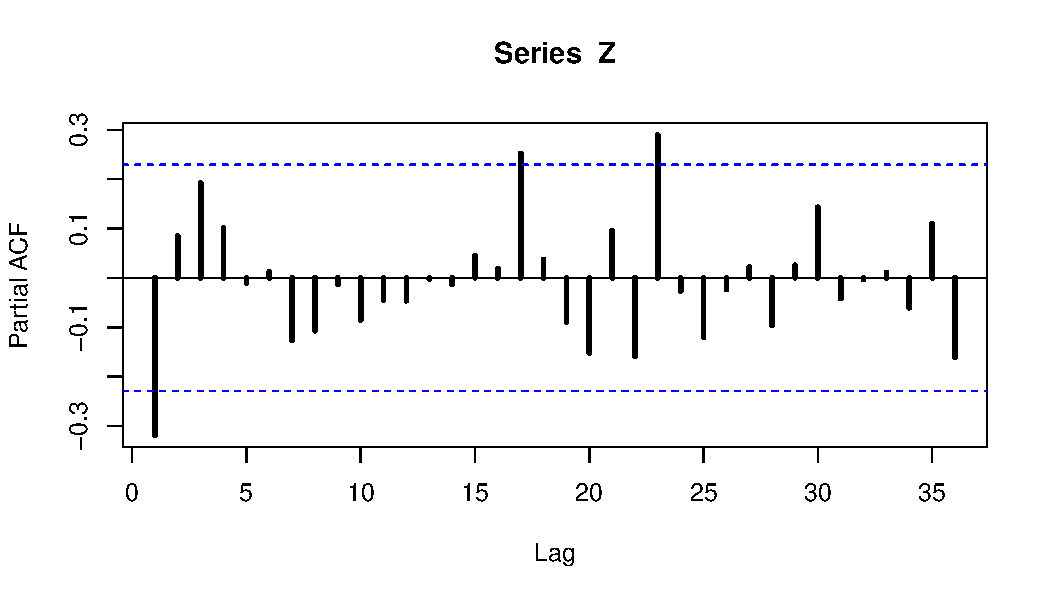
\includegraphics[width=\maxwidth]{figure/pacf} 

\end{knitrout}

Arthur suggests an AR(1)

Create a MA(1) model
\begin{knitrout}
\definecolor{shadecolor}{rgb}{0.969, 0.969, 0.969}\color{fgcolor}\begin{kframe}
\begin{alltt}
model1 <- \hlkwd{arima}(Z, order = \hlkwd{c}(0, 0, 1))
model1
\end{alltt}
\begin{verbatim}
## 
## Call:
## arima(x = Z, order = c(0, 0, 1))
## 
## Coefficients:
##          ma1  intercept
##       -0.237     -583.8
## s.e.   0.092      254.9
## 
## sigma^2 estimated as 8071255:  log likelihood = -684.1,  aic = 1374
\end{verbatim}
\end{kframe}
\end{knitrout}


Create an AR(1) model
\begin{knitrout}
\definecolor{shadecolor}{rgb}{0.969, 0.969, 0.969}\color{fgcolor}\begin{kframe}
\begin{alltt}
model2 <- \hlkwd{arima}(Z, order = \hlkwd{c}(1, 0, 0))
model2
\end{alltt}
\begin{verbatim}
## 
## Call:
## arima(x = Z, order = c(1, 0, 0))
## 
## Coefficients:
##          ar1  intercept
##       -0.321     -583.1
## s.e.   0.111      248.9
## 
## sigma^2 estimated as 7842043:  log likelihood = -683.1,  aic = 1372
\end{verbatim}
\end{kframe}
\end{knitrout}

Arthur goes on to discuss the relative merits of AR(1) and seasonal root models.  The none-stationary model will revel an expanding variance.

\end{document}
